\chapter{Two Dimensions}


In the previous chapter, we solved a one-dimensional problem---a penny falling from the Empire State Building.  Now we'll solve a two-dimensional problem---finding the trajectory of a baseball.

\index{baseball}

To do that, we'll use spatial vectors to represent quantities in two and three dimensions, including force, acceleration, velocity, and position.

\section{Spatial Vectors}
\label{spacial}

The word \emph{vector} means different
things to different people.  In MATLAB, a vector is a matrix that has
either one row or one column.  So far, we've used MATLAB vectors to
represent the following:

\begin{description}

\item[Sequences] A mathematical sequence, like the Fibonacci numbers, is a set of values identified by integer indices; in Chapter~\ref{vecseq}, we used a MATLAB vector to store the elements of a sequence.

\item[State vectors] A state vector is a set of values that
describes the state of a physical system.  When you call
\lstinline{ode45}, you give it initial conditions in a state
vector.  Then, when \lstinline{ode45} calls your rate function, it
gives you a state vector.

\item[Time series] One of the results from \lstinline{ode45} is a vector that represents a sequence of time values.

\end{description}

\index{vector!spatial}
\index{spatial vector}
\index{sequence}
\index{state}
\index{time series}

In this chapter, we'll see another use of MATLAB vectors: representing
\emph{spatial vectors}.  A spatial vector represents a multidimensional physical quantity like position, velocity, acceleration, or force.

\index{position}

For example, to represent a position in two-dimensional space, we can use a vector with two elements:

\begin{code}
>> P = [3 4]
\end{code}

To interpret this vector, we have to know the coordinate system it is defined in.  Most commonly, we use a Cartesian system where the x-axis points east and the y-axis points north.  This is one of many typical conventions, referred to in three dimensions and East-North-Up (ENU). In that case \lstinline{P} represents a point 3~units east and 4~units north of the origin.

\index{Cartesian coordinates}
\index{magnitude}
\index{direction}
\index{Pythagorean theorem}

When a spatial vector is represented in this way, we can use it to compute the magnitude and direction of a physical quantity.
For example,~the \emph{magnitude} of \lstinline{P} is the distance from the origin to \lstinline{P}, which is the hypotenuse of the triangle with sides \lstinline{P(1)} and \lstinline{P(2)}.
We can compute it using the Pytha\-gorean theorem:

\begin{code}
>> sqrt(P(1)^2 + P(2)^2)
ans = 5
\end{code}

Or we can do the same thing using the function \lstinline{norm}, which computes the
\emph{Euclidean norm} of a vector, which is its magnitude:

\index{norm@\lstinline{norm}}
\index{Euclidean norm}

\begin{code}
>> norm(P)
ans = 5
\end{code}

There are two ways to get the \emph{direction} of a vector.  One convention is to compute the angle between the vector and the x-axis:

\begin{code}
>> atan2(P(2), P(1))
ans = 0.9273
\end{code}

In this example, the angle is about \SI{0.9}{\radian}.  But for computational purposes, we often represent direction with a \emph{unit vector}, which is a vector with length~1.  To get a unit vector we can divide a vector by its length:

\begin{code}
function res = hat(V)
    res = V / norm(V)
end
\end{code}

This function takes a vector, \lstinline{V}, and returns a unit vector with the same direction as \lstinline{V}.  It's called \lstinline{hat} because in mathematical notation, unit vectors are written with a ``hat'' symbol.
For example, the unit vector with the same direction as $\vec{P}$ would be written $\uvec{P}$.

\index{unit vector}
\index{vector!unit}

\section{Adding Vectors}

Vectors are useful for representing quantities like force and acceleration because we can add them up without having to think explicitly about direction.

\index{force}
\index{acceleration}

As an example, suppose we have two vectors representing forces:

\begin{code}
>> A = [2, 4];
>> B = [2, -2];
\end{code}

\lstinline{A} represents a force pulling northeast; \lstinline{B} represents a force pulling southeast, as shown in Figure~\ref{fig:vector2}:

\begin{figure}[h]
\centerline{\includegraphics[scale=0.8]{images/figure12_01_new.eps}}
\caption{The sum of two forces represented by vectors}
\label{fig:vector2}
\end{figure}

To compute the sum of these forces, all we have to do is add the vectors:

\begin{code}
>> A + B
ans = 4     2
\end{code}

Later in the chapter, we'll use vector addition to add accelerations due to different forces acting on a baseball.


\section{ODEs in Two Dimensions}
\label{projectile}

So far we've used \lstinline{ode45} to solve a system of first-order equations and a single second-order equation.  Now we'll take one more step, solving a system  of second-order equations.

As an example, we'll simulate the flight of a baseball.
If there is no wind and no spin on the ball, the ball travels in a vertical plane, so we can think of the system as two-dimensional, with $x$ representing the horizontal distance
traveled from the starting place and $y$ representing height or altitude.

\index{baseball}
\index{altitude}
\index{rate function}

Using Newtonian mechanics ($F=ma$), our simple model of the dynamics of a baseball are the following equations of motion:

\begin{eqnarray*}
    \ddot{x}(t) &=& 0 \\
    \ddot{y}(t) &=& -g
\end{eqnarray*}

There are no forces (yet) in the horizontal $x$ direction and only gravity in the vertical $y$ direction.

Using the same process from Section~\ref{s:newton} we can introduce state variable for the velocity of the baseball in the horizontal and vertical direction, $v_x$ and $v_y$.   This process of introducing new variables is confusing at first, but hopefully it makes some intuitive sense that the \emph{state} of our baseball system is described by position and velocity.  The state vector of the system is then these four states.  They can be in any order.  The order is important to keep in mind for book keeping in implementation, but the physics don't change.  We'll choose to define the state vector as
\begin{equation}\label{e:bstate}
    \mathbf{x}(t) = \left\{ \begin{array}{c}
        x \\ v_x  \\ y \\ v_y
    \end{array}\right\}.
\end{equation}

The model, now in state-space from, becomes
\begin{equation}\label{e:baseballstate}
    \left\{ \begin{array}{c}
        \dot{x}(t) \\ \dot{v_x}(t)  \\ \dot{y}(t) \\ \dot{v_y}(t)
    \end{array}\right\}
    =
    \left[ \begin{array}{cccc}
        0  & 1 & 0 & 0\\
        0 & 0 & 0 & 0\\
        0 & 0 & 0 & 1\\
        0 & 0 & 0 & 0\\
    \end{array}
    \right]
    \left\{ \begin{array}{c}
        x \\ v_x  \\ y \\ v_y
    \end{array}\right\}
    +
    \left\{\begin{array}{c}
         0 \\ 0 \\ 0 \\ -g
    \end{array}
    \right\}
    .
\end{equation}

Listing~\ref{lst:baseball_rate_func} shows a rate function, named \lstinline{state_transition}, we can use to simulate this system with \lstinline{ode45}:

\lstinputlisting[style=mcode, firstline=31, lastline=58, caption={A rate function we can use to model the flight of a baseball}, label={lst:baseball_rate_func}]
{../code/chap_twodimensions/baseball_statespace.m}

The second argument of is understood to be a vector,\lstinline{xx}, with four elements.  To avoid a hard-to-find semantic bug, it is key that you use a consistent interpretation of the meaning of this vector, that it includes the variables in the order that we defined in Equation~\ref{ebstate}.  Having a written mathematical model, Equation~\ref{e:baseballstate}, is a good defense.

The goal of the rate function is to compute the derivative of the state vector \lstinline{xx}, the left-hand side of Equation\~ref{e:baseballstate}.   

For now, we'll ignore air resistance, so the only force on the baseball is gravity.  We represent acceleration due to gravity with a vector that has magnitude \lstinline{g} and direction along the negative y-axis.

Let's assume that a ball is batted from an initial position \SI{1}{\meter} above the home plate, with an initial velocity of \SI{40}{\meter\per\second} in the horizontal and \SI{30}{\meter\per\second} in the vertical direction.

\index{initial condition}

Here's how we can call \lstinline{ode45} with these initial conditions:

\lstinputlisting[style=mcode, firstline=1, lastline=30]{../code/chap_twodimensions/baseball_statespace.m}

The initial conditions are defined by \lstinline{xx_init} as a column vector using the transpose operator \lstinline{'}.

The output variables from \lstinline{ode45} are a vector, \lstinline{tout}, that contains time values and a matrix, \lstinline{Xout}, with four columns.  Each row of \lstinline{Xout} is the state of the system at the corresponding time from \lstinline{tout}.  We can slice this matrix to access the position values based on our model's definition of state, Equation~\ref{e:bstate}.


Figure~\ref{f:baseball1} shows what these coordinates look like as a function of time and in space.  The x-coordinate increases linearly because the $x$ velocity is constant.  The y-coordinate goes up and down, as we expect.

\begin{figure}[h]
    \centering
    \begin{subfigure}{0.45\textwidth}
        \centering
        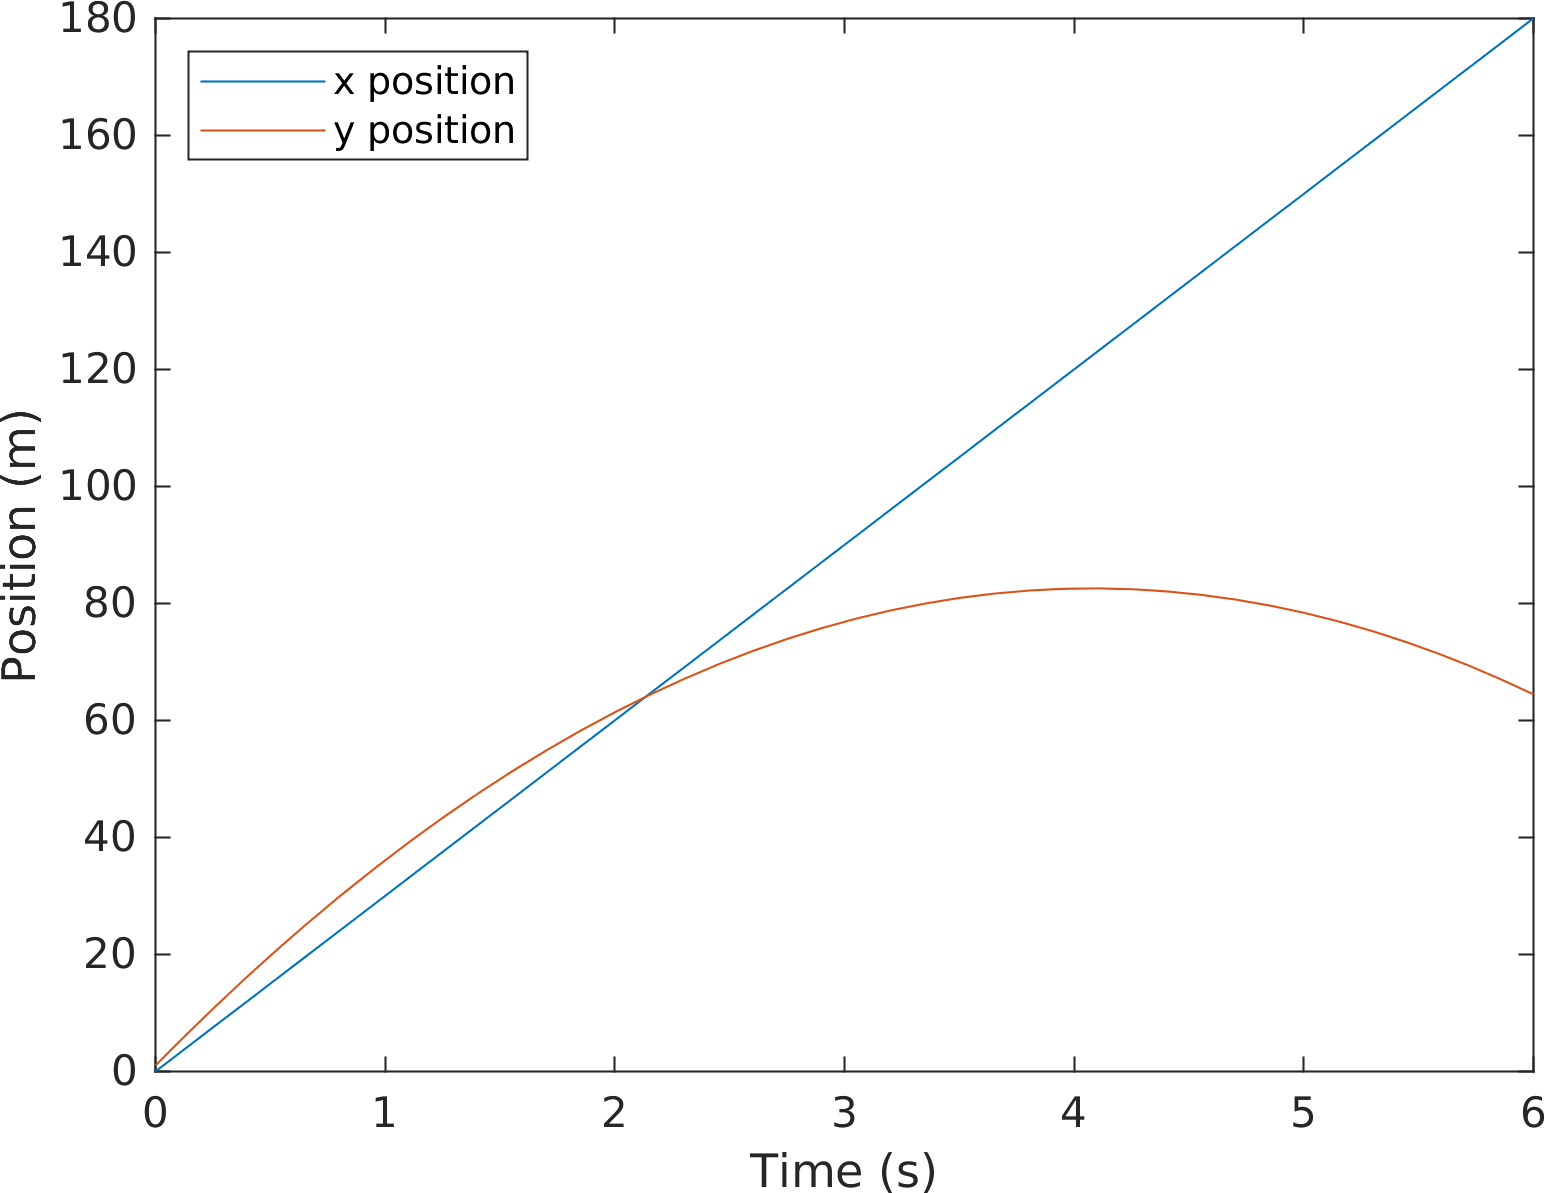
\includegraphics[width=\linewidth]{../code/chap_twodimensions/baseball_time.png}
        \caption{Baseball solution time series}
    \end{subfigure}
    \quad % Adds some horizontal space between the images
    \begin{subfigure}{0.45\textwidth}
        \centering
        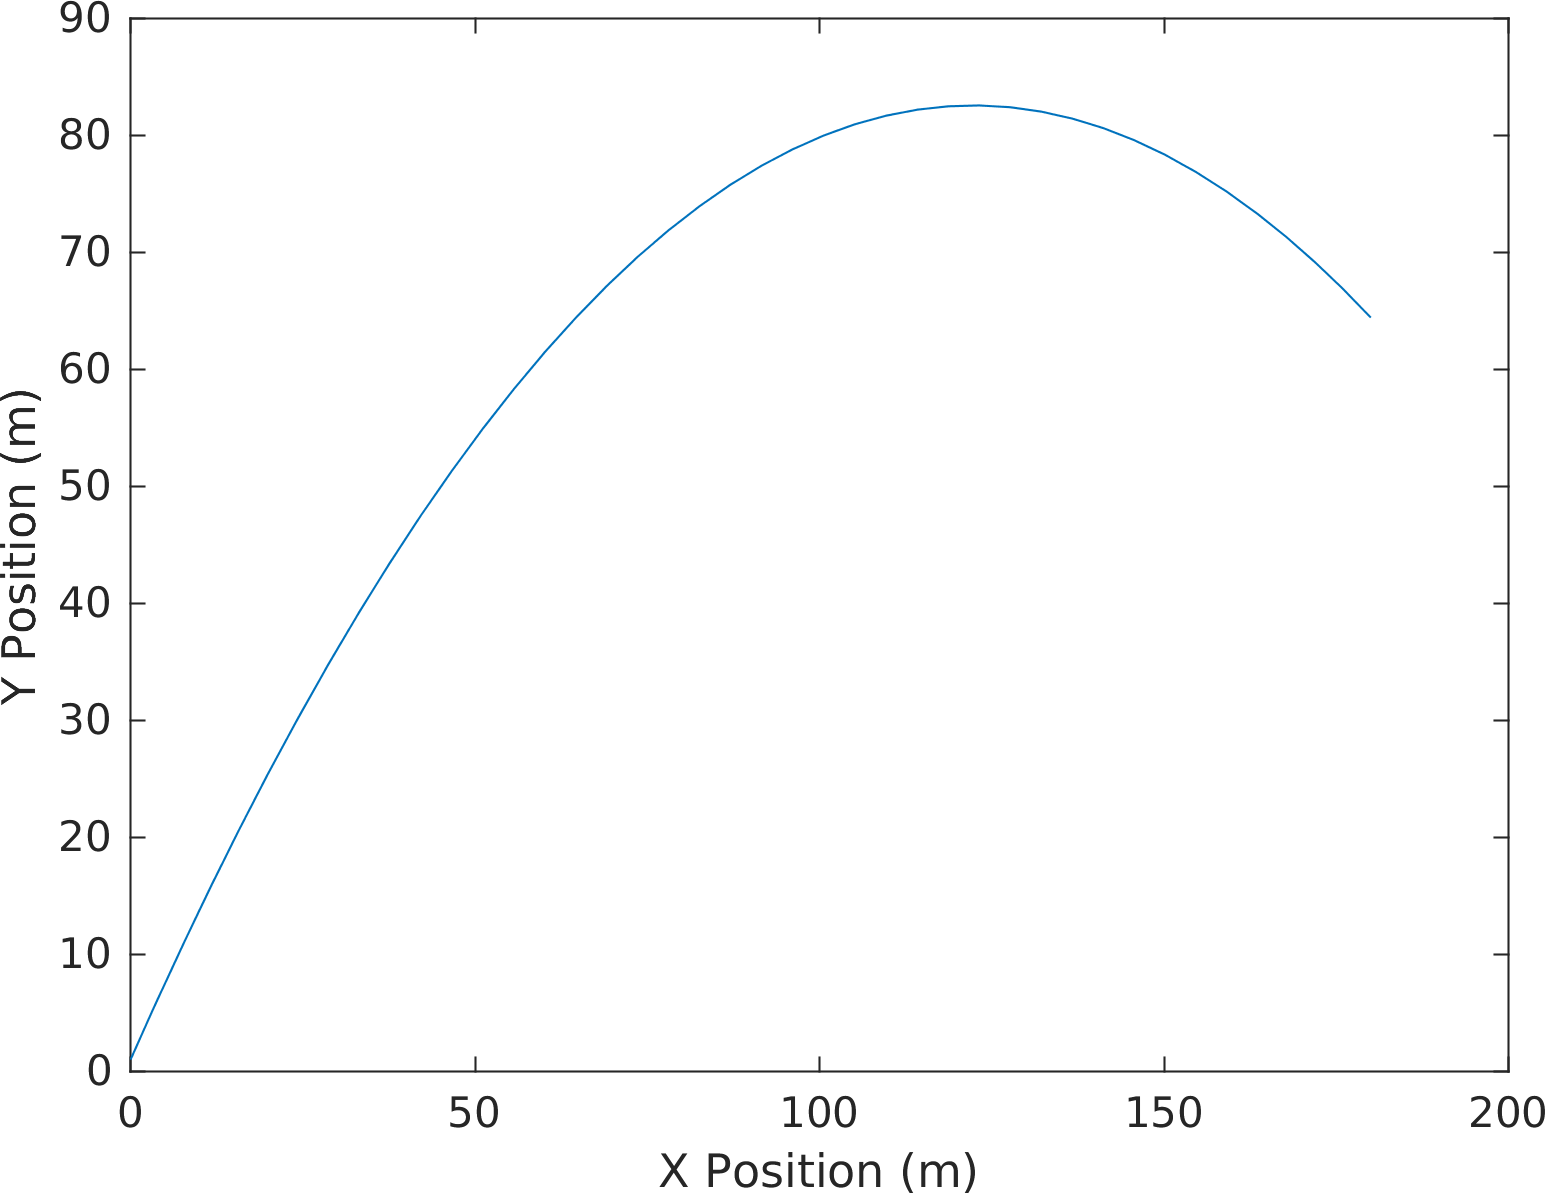
\includegraphics[width=\linewidth]{../code/chap_twodimensions/baseball_xy.png}
        \caption{Baseball solution in x and y}
    \end{subfigure}
    \caption{Two ways to visualize the solution}
    \label{f:baseball1}
\end{figure}

The simulation ends just before the ball lands, having traveled almost \SI{180}{\meter}.  That's substantially farther than a real baseball would travel, because we have ignored air resistance, or ``drag force.''

\section{Drag Force}
\label{drag}

\index{drag}
\index{force!drag}

A simple model for the drag force on a baseball is

\begin{equation*}
    \vec{F}_\mathrm{d} = - \frac{1}{2} \, \rho v C_\mathrm{d} A \uvec{V}
\end{equation*}
where $\vec{F}_\mathrm{d}$ is a vector that represents the force on the baseball
due to drag,
$\rho$ is the density of air,
$C_\mathrm{d}$ is the drag coefficient, and
$A$ is the cross-sectional area.

\index{drag coefficient}
\index{coefficient!drag}

$\vec{V}$ is the baseball's velocity vector, $v$ is the magnitude of $\vec{V}$, and $\uvec{V}$ is a unit vector in the same direction as $\vec{V}$.  The minus sign at the beginning means that the result is in the opposite direction to $\vec{V}$.

\index{unit vector}

The function in Listing~\ref{lst:baseball_drag} computes the drag force on a baseball:
\lstinputlisting[style=mcode, firstline=68, lastline=81, label=lst:baseball_drag]{../code/chap_twodimensions/baseball_statespace2.m}


The drag coefficient for a baseball is about 0.3.
The density of air at sea level is about \SI{1.3}{\kilogram\per\meter\cubed}.
The cross-sectional area of a baseball is \SI{0.0042}{\meter\squared}.

\index{density}
\index{cross-sectional area}

Now we have to update \lstinline{acceleration} to take drag into account:
\lstinputlisting[style=mcode, firstline=51, lastline=67]{../code/chap_twodimensions/baseball_statespace2.m}


As in Listing~\ref{lst:baseball_rate_func}, \lstinline{acceleration} represents acceleration due to gravity with a vector that has magnitude \lstinline{g} and direction along the negative y-axis.
But now it also computes drag force and divides by the mass of the baseball to get acceleration due to drag.
Finally, it adds the two acceleration vectors, representing gravity and drag, to get the total acceleration of the baseball.


Figure~\ref{fig:vector3} shows the following quantities graphically:  (1) acceleration due to drag, $\vec{D}$, which is in the opposite direction to (2)~velocity, $\vec{V}$; (3)~acceleration due to gravity, $\vec{G}$, which is straight down; and (4)~total acceleration, $\vec{A}$, which is the sum of $\vec{D}$ and $\vec{G}$.

\begin{figure}[h]
\centerline{\includegraphics[scale=0.8]{images/figure12_03_new.eps}}
\caption{Diagram of velocity, $\vec{V}$; acceleration due to drag force,
$\vec{D}$; acceleration due to gravity, $\vec{G}$; and total acceleration, $\vec{A}$}
\label{fig:vector3}
\end{figure}

\index{acceleration}

Figure~\ref{f:baseball2} shows the results from \lstinline{ode45}.  The ball lands after about \SI{5}{\second}, having traveled less than \SI{120}{\meter}, substantially less than what we got without air resistance, about \SI{180}{\meter}.


\begin{figure}[h]
    \centering
    \begin{subfigure}{0.45\textwidth}
        \centering
        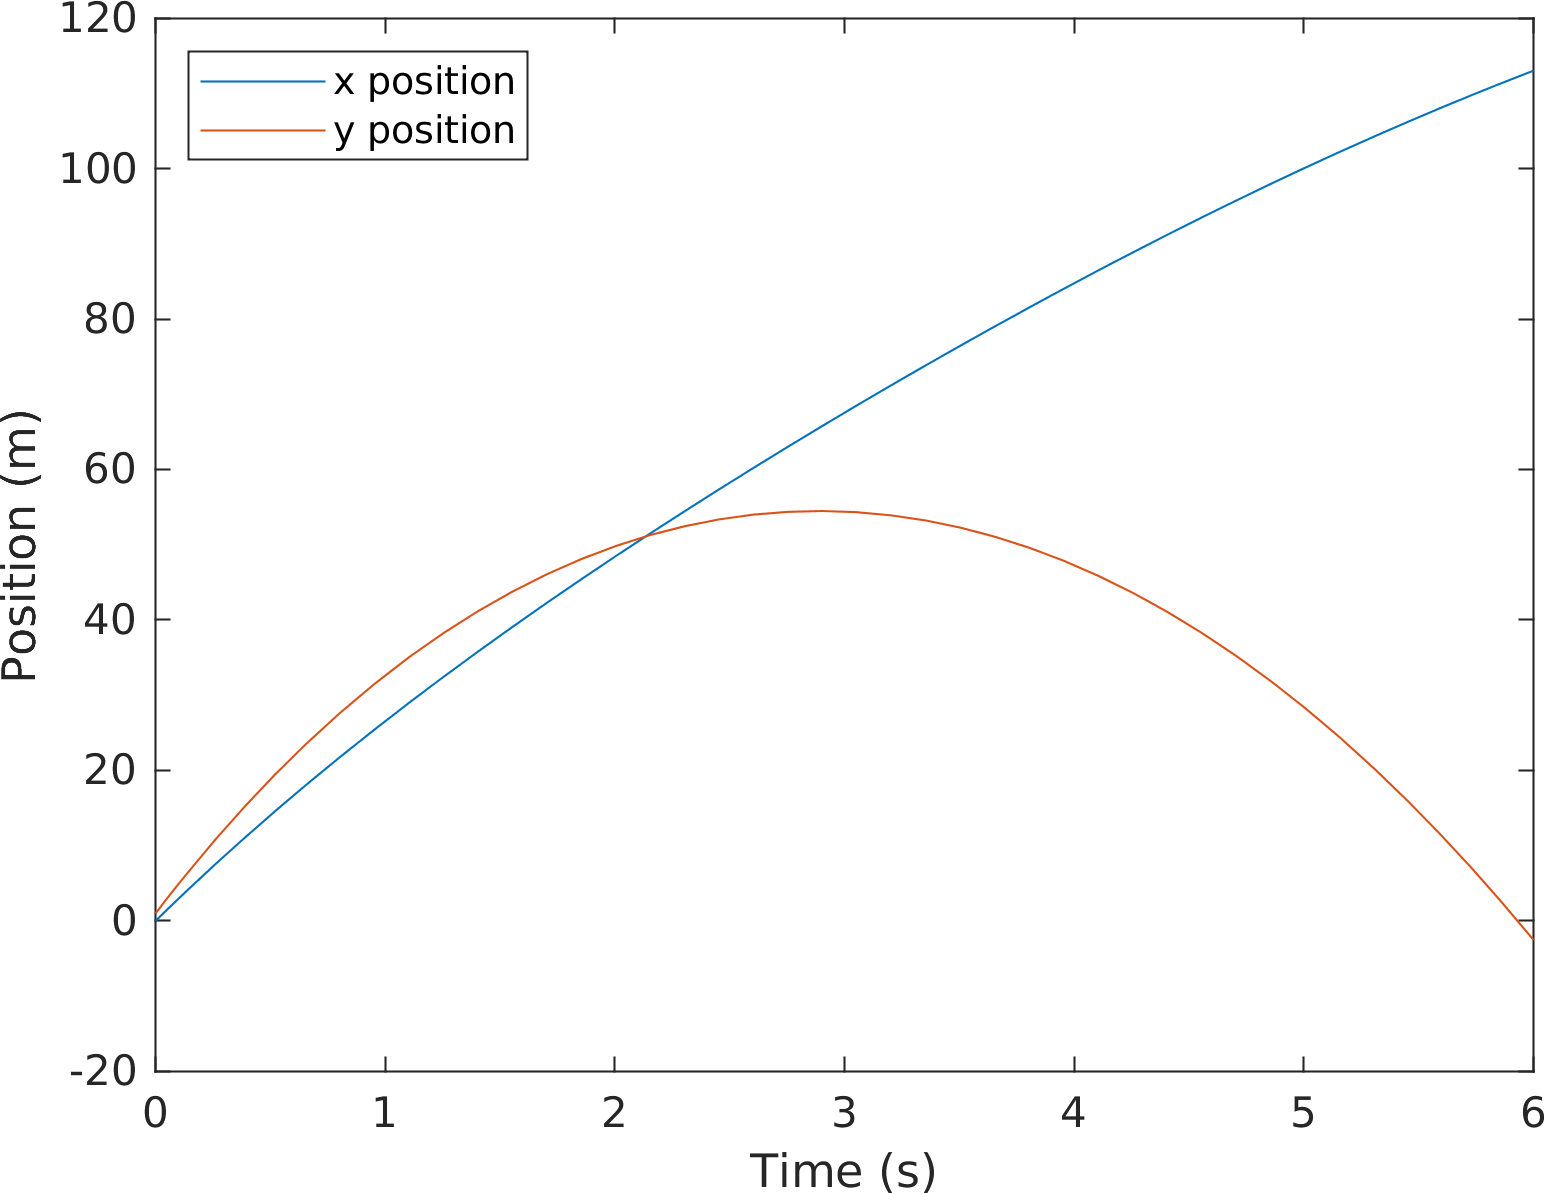
\includegraphics[width=\linewidth]{../code/chap_twodimensions/baseball2_time.png}
        \caption{Baseball solution time series}
    \end{subfigure}
    \quad % Adds some horizontal space between the images
    \begin{subfigure}{0.45\textwidth}
        \centering
        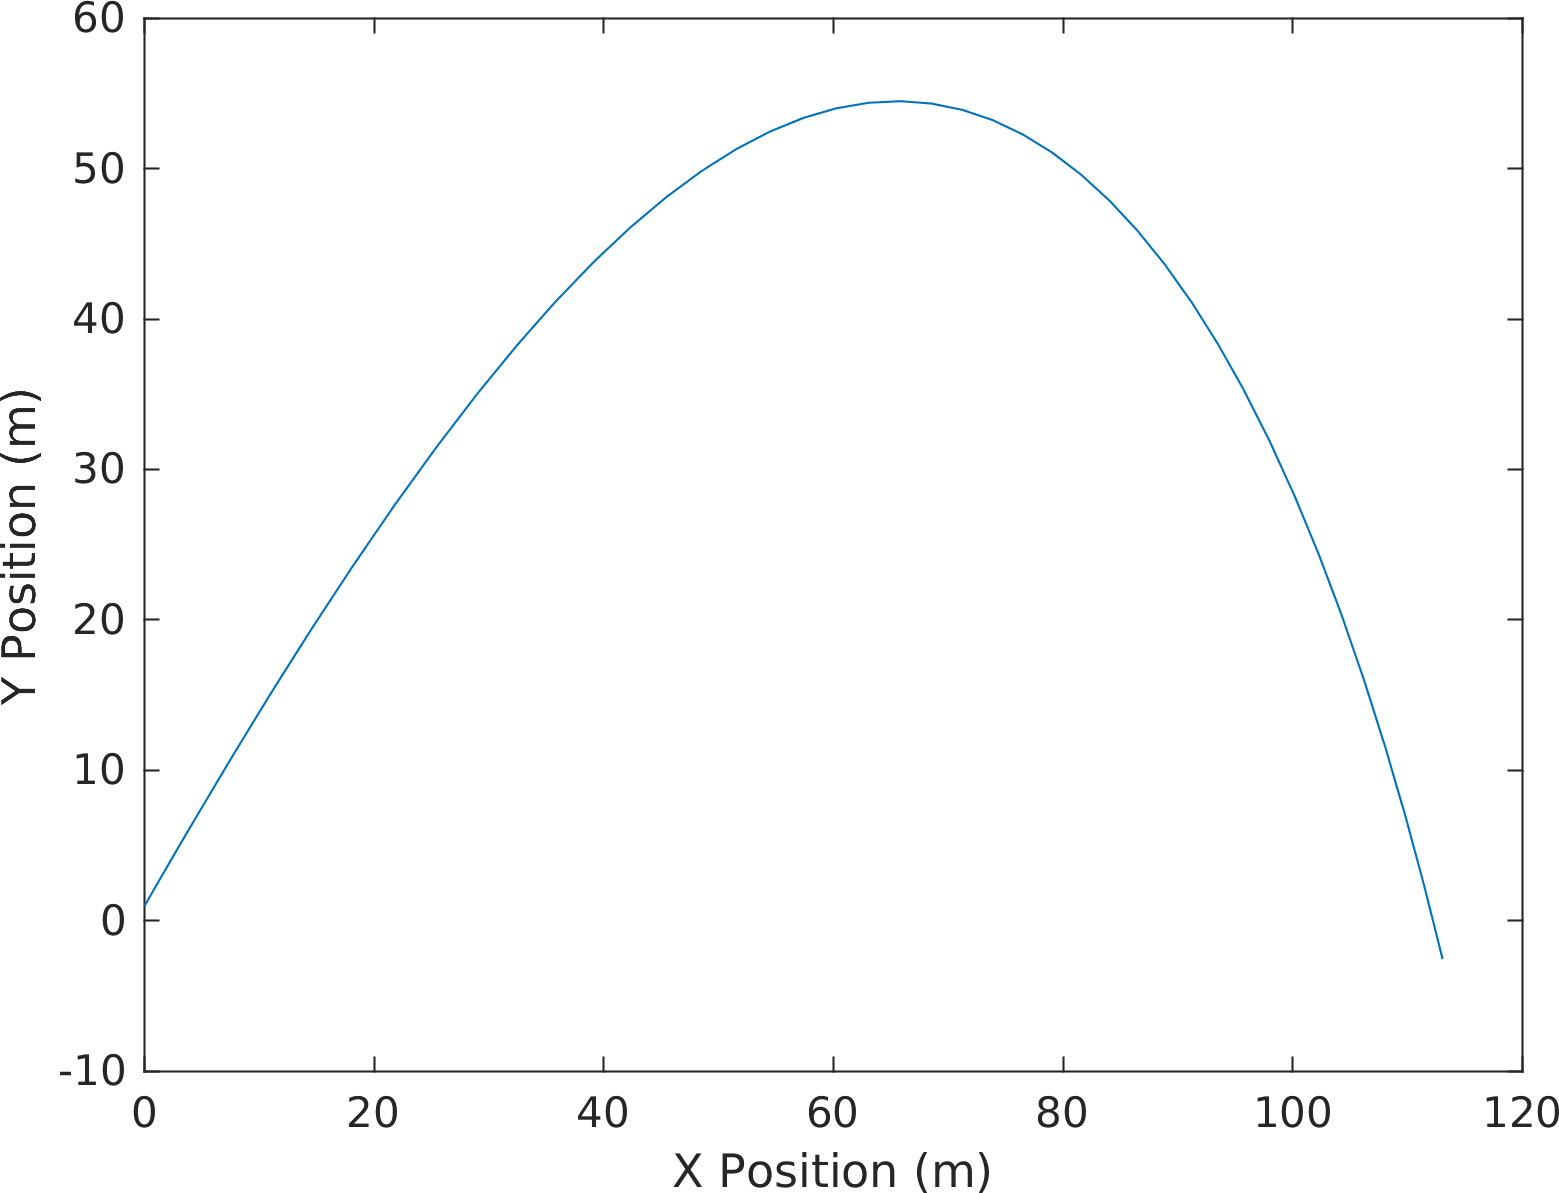
\includegraphics[width=\linewidth]{../code/chap_twodimensions/baseball2_xy.png}
        \caption{Baseball solution in x and y}
    \end{subfigure}
    \caption{Simulated flight of a baseball including drag force including drag froce}
    \label{f:baseball2}
\end{figure}

This result suggests that ignoring air resistance is not a good choice for modeling a baseball.

\section{Chapter Review}

In this chapter, we simulated the flight of a baseball with and without air resistance and saw that the difference is substantial.
We can conclude that it's important to model air resistance if we want to make accurate predictions about baseballs and similar projectiles.

Here are some terms from this chapter you might want to remember.

A \emph{spatial vector} is a value that represents a multidimensional physical quantity like position, velocity, acceleration, or force.
A spatial vector has a direction and a magnitude.  The magnitude is also called the \emph{norm} of the vector.
A \emph{unit vector} is a vector with norm 1, which is often used to represent a
direction.

In the next chapter, we'll continue with the baseball example, using \lstinline{fzero}, which we saw in Chapter~\ref{fzero}, and a new tool for optimization, called \lstinline{fminsearch}.  We'll also see a simple way to animate the solution of a differential equation.


\section{Exercises}

Before you go on, you might want to work on the following exercises.

\begin{ex}

\index{Boston Red Sox}
\index{density}

When the Boston Red Sox won the World Series in 2007, they played the
Colorado Rockies at their home field in Denver, Colorado.  Find an
estimate of the density of air in the Mile High City.  What effect
does this have on drag?  What effect does it have on the distance the baseball travels?
\end{ex}


\begin{ex}

\index{drag}
\index{air resistance}
\index{coefficient!drag}

The actual drag on a baseball is more complicated than what is
captured by our simple model.  In particular, the drag coefficient
depends on velocity.  You can get some of the details from Robert~K.\ Adair's \emph{The
Physics of Baseball} (Harper Perennial, 2002); the figure you need is reproduced at \url{https://greenteapress.com/matlab/drag}.

Use this data to specify a more realistic model of drag and modify your
program to implement it.  How big is the effect on the distance the baseball travels?
\end{ex}


\begin{ex}
\label{cannon}

\index{cannon}
\index{human cannonball}

According to Wikipedia, the record distance for a human cannonball is \SI {59.05}{\meter} (see \url{https://greenteapress.com/matlab/cannon}).

Modify the example from this chapter to simulate the flight of a human cannonball.  You might have to do some research to find the drag coefficient and cross-sectional area for a flying human.

Find the initial velocity (both magnitude and direction) you would need to break this record.  You might have to experiment to find the optimal launch angle.

How much acceleration can a human withstand without injury?  At this maximum acceleration, how long would the barrel of the cannon have to be to reach the initial velocity needed to break the record?

\end{ex}
